\documentclass[oneside,openany,headings=optiontotoc,11pt,numbers=noenddot]{scrreprt}

\usepackage[a4paper]{geometry}
\usepackage[utf8]{inputenc}
\usepackage[T1]{fontenc}
\usepackage{lmodern}
\usepackage[ngerman]{babel}
\usepackage{ngerman}

\usepackage[onehalfspacing]{setspace}

\usepackage{fancyhdr}
\usepackage{fancybox}

\usepackage{rotating}
\usepackage{varwidth}

%Struktogramme
\usepackage[german,curves]{struktex}

\usepackage{pdflscape}
\usepackage{changepage}
\usepackage{graphicx}
\usepackage[bottom]{footmisc}
\usepackage{transparent}
\usepackage{graphbox}
\graphicspath{
	{Pics/PDFs/}
	{Pics/JPGs/}
	{Pics/PNGs/}
}
\usepackage{caption}
\usepackage{wrapfig}
\usepackage{marginnote}
\usepackage{tabularx}
\usepackage{dashrule}
\usepackage{soulutf8}
\usepackage{hhline}
%arydshln suppresses vertical lines in table
%\usepackage{arydshln}
\usepackage{multirow}
\usepackage{enumerate}
\usepackage[hidelinks]{hyperref}
\usepackage{listings}

\usepackage[table]{xcolor}
\usepackage{array}
\usepackage{enumitem,amssymb,amsmath}
\usepackage{interval}
\usepackage{cancel}
\usepackage{stmaryrd}
\usepackage{wasysym}
\usepackage{polynom}
\usepackage{diagbox}
\usepackage{dashrule}
\usepackage{framed}
\usepackage{mdframed}
\usepackage{karnaugh-map}
\usepackage{pdfpages}

\usepackage{blindtext}

\usepackage{eso-pic}

\usepackage{amssymb}
\usepackage{eurosym}

\usepackage[pages=some]{background}
\pagestyle{headings}
\renewcommand{\headrulewidth}{0.2pt}
\renewcommand{\footrulewidth}{0.2pt}
\newcommand*{\underdownarrow}[2]{\ensuremath{\underset{\overset{\Big\downarrow}{#2}}{#1}}}
\setlength{\fboxsep}{5pt}
\newcommand{\explainBelow}[3]{\underbrace{#1}_{\parbox{\widthof{#3}}{\footnotesize\raggedright #2}}}
\newcommand{\explainAbove}[3]{\overbrace{#1}^{\parbox{\widthof{#3}}{\footnotesize\raggedright #2}}}
\newcommand\footnoteref[1]{\protected@xdef\@thefnmark{\ref{#1}}\@footnotemark}


% Codestyle defined
\definecolor{codegreen}{rgb}{0,0.6,0}
\definecolor{codegray}{rgb}{0.5,0.5,0.5}
\definecolor{codepurple}{rgb}{0.58,0,0.82}
\definecolor{backcolour}{rgb}{0.95,0.95,0.92}
\definecolor{deepgreen}{rgb}{0,0.5,0}
\definecolor{darkblue}{rgb}{0,0,0.65}
\definecolor{mauve}{rgb}{0.40, 0.19,0.28}
\colorlet{exceptioncolour}{yellow!50!red}
\colorlet{commandcolour}{blue!60!black}
\colorlet{numpycolour}{blue!60!green}
\colorlet{specmethodcolour}{violet}

%Neue Spaltendefinition
\newcolumntype{L}[1]{>{\raggedright\let\newline\\\arraybackslash\hspace{0pt}}m{#1}}
\newcolumntype{M}{>{\centering\arraybackslash}X}
\newcommand{\cmnt}[1]{\ignorespaces}
%Textausrichtung ändern
\newcommand\tabrotate[1]{\rotatebox{90}{\raggedright#1\hspace{\tabcolsep}}}

%Intervall-Konfig
\intervalconfig {
	soft open fences
}

%Bash
\lstdefinestyle{BashInputStyle}{
	language=bash,
	basicstyle=\small\sffamily,
	backgroundcolor=\color{backcolour},
	columns=fullflexible,
	backgroundcolor=\color{backcolour},
	breaklines=true,
}
%Java
\lstdefinestyle{JavaInputStyle}{
	language=Java,
	backgroundcolor=\color{backcolour},
	aboveskip=1mm,
	belowskip=1mm,
	showstringspaces=false,
	columns=flexible,
	basicstyle={\footnotesize\ttfamily},
	numberstyle={\tiny},
	numbers=none,
	keywordstyle=\color{purple},,
	commentstyle=\color{deepgreen},
	stringstyle=\color{blue},
	emph={out},
	emphstyle=\color{darkblue},
	emph={[2]rand},
	emphstyle=[2]\color{specmethodcolour},
	breaklines=true,
	breakatwhitespace=true,
	tabsize=2,
}
%Python
\lstdefinestyle{PythonInputStyle}{
	language=Python,
	alsoletter={1234567890},
	aboveskip=1ex,
	basicstyle=\footnotesize,
	breaklines=true,
	breakatwhitespace= true,
	backgroundcolor=\color{backcolour},
	commentstyle=\color{red},
	otherkeywords={\ , \}, \{, \&,\|},
	emph={and,break,class,continue,def,yield,del,elif,else,%
		except,exec,finally,for,from,global,if,import,in,%
		lambda,not,or,pass,print,raise,return,try,while,assert},
	emphstyle=\color{exceptioncolour},
	emph={[2]True,False,None,min},
	emphstyle=[2]\color{specmethodcolour},
	emph={[3]object,type,isinstance,copy,deepcopy,zip,enumerate,reversed,list,len,dict,tuple,xrange,append,execfile,real,imag,reduce,str,repr},
	emphstyle=[3]\color{commandcolour},
	emph={[4]ode, fsolve, sqrt, exp, sin, cos, arccos, pi,  array, norm, solve, dot, arange, , isscalar, max, sum, flatten, shape, reshape, find, any, all, abs, plot, linspace, legend, quad, polyval,polyfit, hstack, concatenate,vstack,column_stack,empty,zeros,ones,rand,vander,grid,pcolor,eig,eigs,eigvals,svd,qr,tan,det,logspace,roll,mean,cumsum,cumprod,diff,vectorize,lstsq,cla,eye,xlabel,ylabel,squeeze},
	emphstyle=[4]\color{numpycolour},
	emph={[5]__init__,__add__,__mul__,__div__,__sub__,__call__,__getitem__,__setitem__,__eq__,__ne__,__nonzero__,__rmul__,__radd__,__repr__,__str__,__get__,__truediv__,__pow__,__name__,__future__,__all__},
	emphstyle=[5]\color{specmethodcolour},
	emph={[6]assert,range,yield},
	emphstyle=[6]\color{specmethodcolour}\bfseries,
	emph={[7]Exception,NameError,IndexError,SyntaxError,TypeError,ValueError,OverflowError,ZeroDivisionError,KeyboardInterrupt},
	emphstyle=[7]\color{specmethodcolour}\bfseries,
	emph={[8]taster,send,sendMail,capture,check,noMsg,go,move,switch,humTem,ventilate,buzz},
	emphstyle=[8]\color{blue},
	keywordstyle=\color{blue}\bfseries,
	rulecolor=\color{black!40},
	showstringspaces=false,
	stringstyle=\color{deepgreen}
}

\lstset{literate=%
	{Ö}{{\"O}}1
	{Ä}{{\"A}}1
	{Ü}{{\"U}}1
	{ß}{{\ss}}1
	{ü}{{\"u}}1
	{ä}{{\"a}}1
	{ö}{{\"o}}1
}

% Neue Klassenarbeits-Umgebung
\newenvironment{worksheet}[3]
% Begin-Bereich
{
	\newpage
	\sffamily
	\setcounter{page}{1}
	\ClearShipoutPicture
	\AddToShipoutPicture{
		\put(55,761){{
				\mbox{\parbox{385\unitlength}{\tiny \color{codegray}BBS I Mainz, #1 \newline #2
						\newline #3
					}
				}
			}
		}
		\put(455,761){{
				\mbox{\hspace{0.3cm}
\includegraphics[width=0.2\textwidth]{../../logo.pdf}}
			}
		}
	}
}
% End-Bereich
{
	\clearpage
	\ClearShipoutPicture
}

\geometry{left=2.00cm,right=1.50cm,top=3.00cm,bottom=1.00cm,includeheadfoot}

\begin{document}
	\begin{test}{Vorbereitung}{Mathematik}{HBF IT 18A - V}
		\begin{framed}
			\noindent
			\scriptsize{Allgemeines
			\begin{itemize}[noitemsep,topsep=0pt]
				\item[-] Bei der Bearbeitung ist ein \textbf{nachvollziehbarer, vollständiger Rechenweg} aufzuschreiben.
				\item[-] Die Bewertung der Klassenarbeit ist nur bei \textbf{gut lesbarer Schrift} möglich.
				\item[-] Die Lösungen müssen mit dokumentenechtem Stift (\textbf{Kugelschreiber} oder \textbf{Fine-Liner} - keine rote Mine) erstellt werden.
				\item[-] Runden Sie ihre Ergebnisse auf \textbf{2 Nachkommastellen}. Wurzelausdrücke müssen nicht berechnet werden (z.B. \(\sqrt{10}\)).\\
				
				\item[-] \textbf{Zugelassene Hilfsmittel}: Taschenrechner (nicht graphikfähig / programmierbar)
				\item[-] \textbf{Bearbeitungszeit:} 90 Minuten
			\end{itemize}}
		\end{framed}
		\normalsize
			\noindent
		\begin{tabularx}{\textwidth}{Xl}\underline{\textbf{Aufgabe 1}}& \end{tabularx}\\
		\par\noindent
		Gegeben ist die nachfolgende Funktion: \[f(x) = -0,5x^3 + 2x^2 + 3x - 4\]
		\begin{itemize}
			\item[(a)] \textbf{Geben} Sie den \underline{charakteristischen Summanden} sowie den \underline{y-Achsenabschnitt} an.
			\item[(b)] \textbf{Treffen} Sie eine Aussage über das Verhalten der Funktion für große x-Beträge.\\
			\footnotesize{\textit{Hinweis}: Nutzen Sie die Notation \(f(x)\xrightarrow{x\rightarrow-\infty}\) und \(f(x)\xrightarrow{x\rightarrow\infty}\)}\normalsize
			\item[(c)] \textbf{Endscheiden} und \textbf{begründen} Sie, ob der Funktionsgraph symmetrisch ist.
			\item[(d)] Wie müsste die Funktion verändert werden, um eine Symmetrie zu erhalten?
		\end{itemize}
		\par\noindent
		\begin{tabularx}{\textwidth}{Xl}\underline{\textbf{Aufgabe 2}}&\end{tabularx}\\
		Beschreiben Sie das \textbf{Verhalten} der folgenden Funktionen \textbf{für große x-Beträge}.
		\begin{itemize}
			\item[(a)] \(f(x) = 5x^{3} + 500x^{2} - 30\)
			\item[(b)] \(f(x) = -0.2x^{4} - 2x^{3} - 5x^{2} - x + 2\)
			\item[(c)] \(f(x) = -10x^{7} + 8x^{5} - 6x^{3} + 1\)
			\item[(d)] \(f(x) = 25x^{4} + 20x^{3} - 14x + 500\)
		\end{itemize}
		\noindent
		\begin{tabularx}{\textwidth}{Xl}\underline{\textbf{Aufgabe 3}}&\end{tabularx}\\
		(I) \textbf{Überführen} Sie die in \underline{Polynomform} gegebene Funktion in die \underline{Linearfaktorform}.\\
		\par\noindent
		\begin{tabularx}{\textwidth}{MM}
			(a) \(f(x) = x^3 - 3x^2 +4\) & (b) \(g(x) = x^4 -4x^2 + 4\)
		\end{tabularx}\\
		\par\noindent
		\footnotesize{\textit{Hinweis:} Sie benötigen die Nullstellen.}\\
		\rule{\textwidth}{0.1pt}\\
		\par\noindent
		\normalsize
		(II) \textbf{Überführen} Sie \(\mathbf{f(x) = (x^2 - 3)(x+2)^2}\) in die \underline{Polynomform}.
		\par\noindent
	\end{test}
	\newgeometry{left=2.00cm,right=1.50cm,top=1.50cm,bottom=1.00cm,includeheadfoot}
	\noindent
	\begin{tabularx}{\textwidth}{Xl}\underline{\textbf{Aufgabe 4}}&\end{tabularx}\\
	Ordnen Sie die Graphen der Steigungsfunktionen den richtigen Ausgangsgraphen für \(f(x)\) zu.\\
	\textbf{Begründen} Sie ihre Entscheidung in Stichpunkten.\\
	\begin{tabularx}{\textwidth}{|cX|cX|cX|}
		\hline
		\multicolumn{6}{|l|}{Ausgangsgraph von \(f(x)\)}\\
		\hline
		(a) & & (b) & & (c) &\\
		& 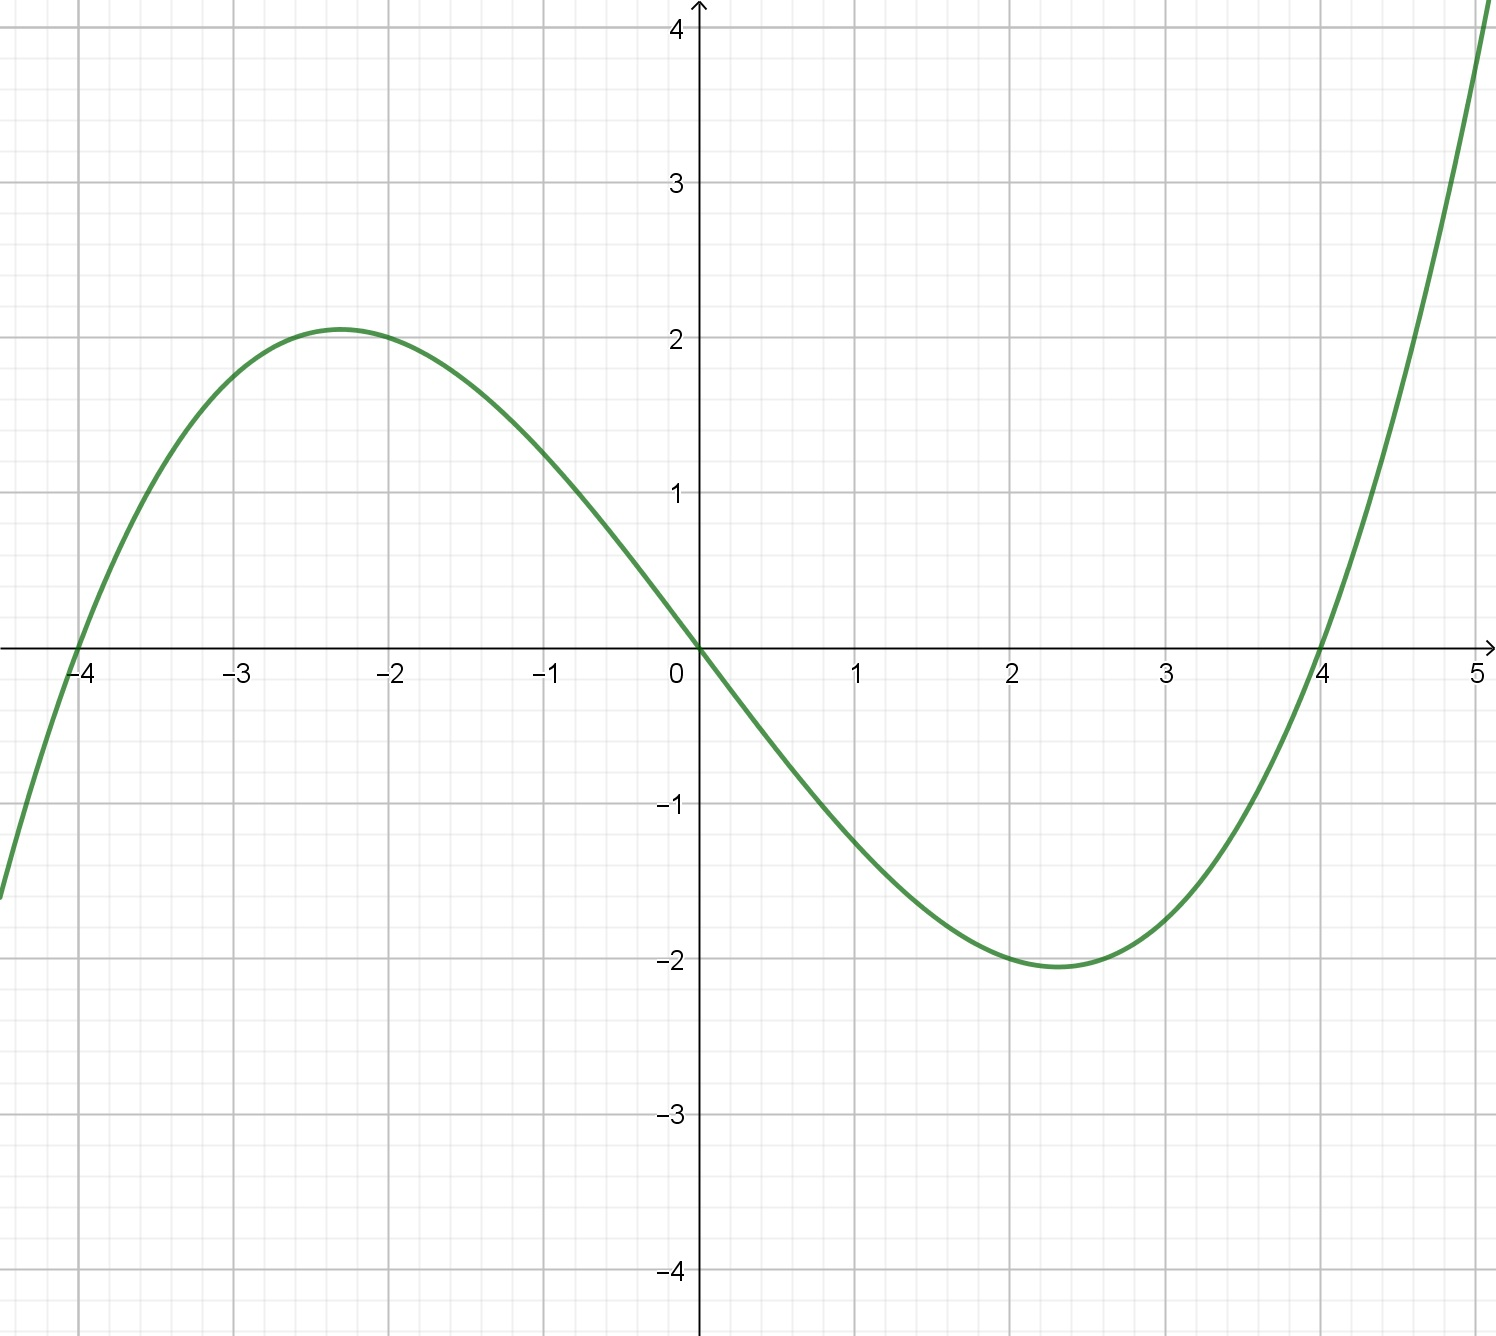
\includegraphics[scale=0.14]{../99_Bilder/3VKA/a.jpg} & & 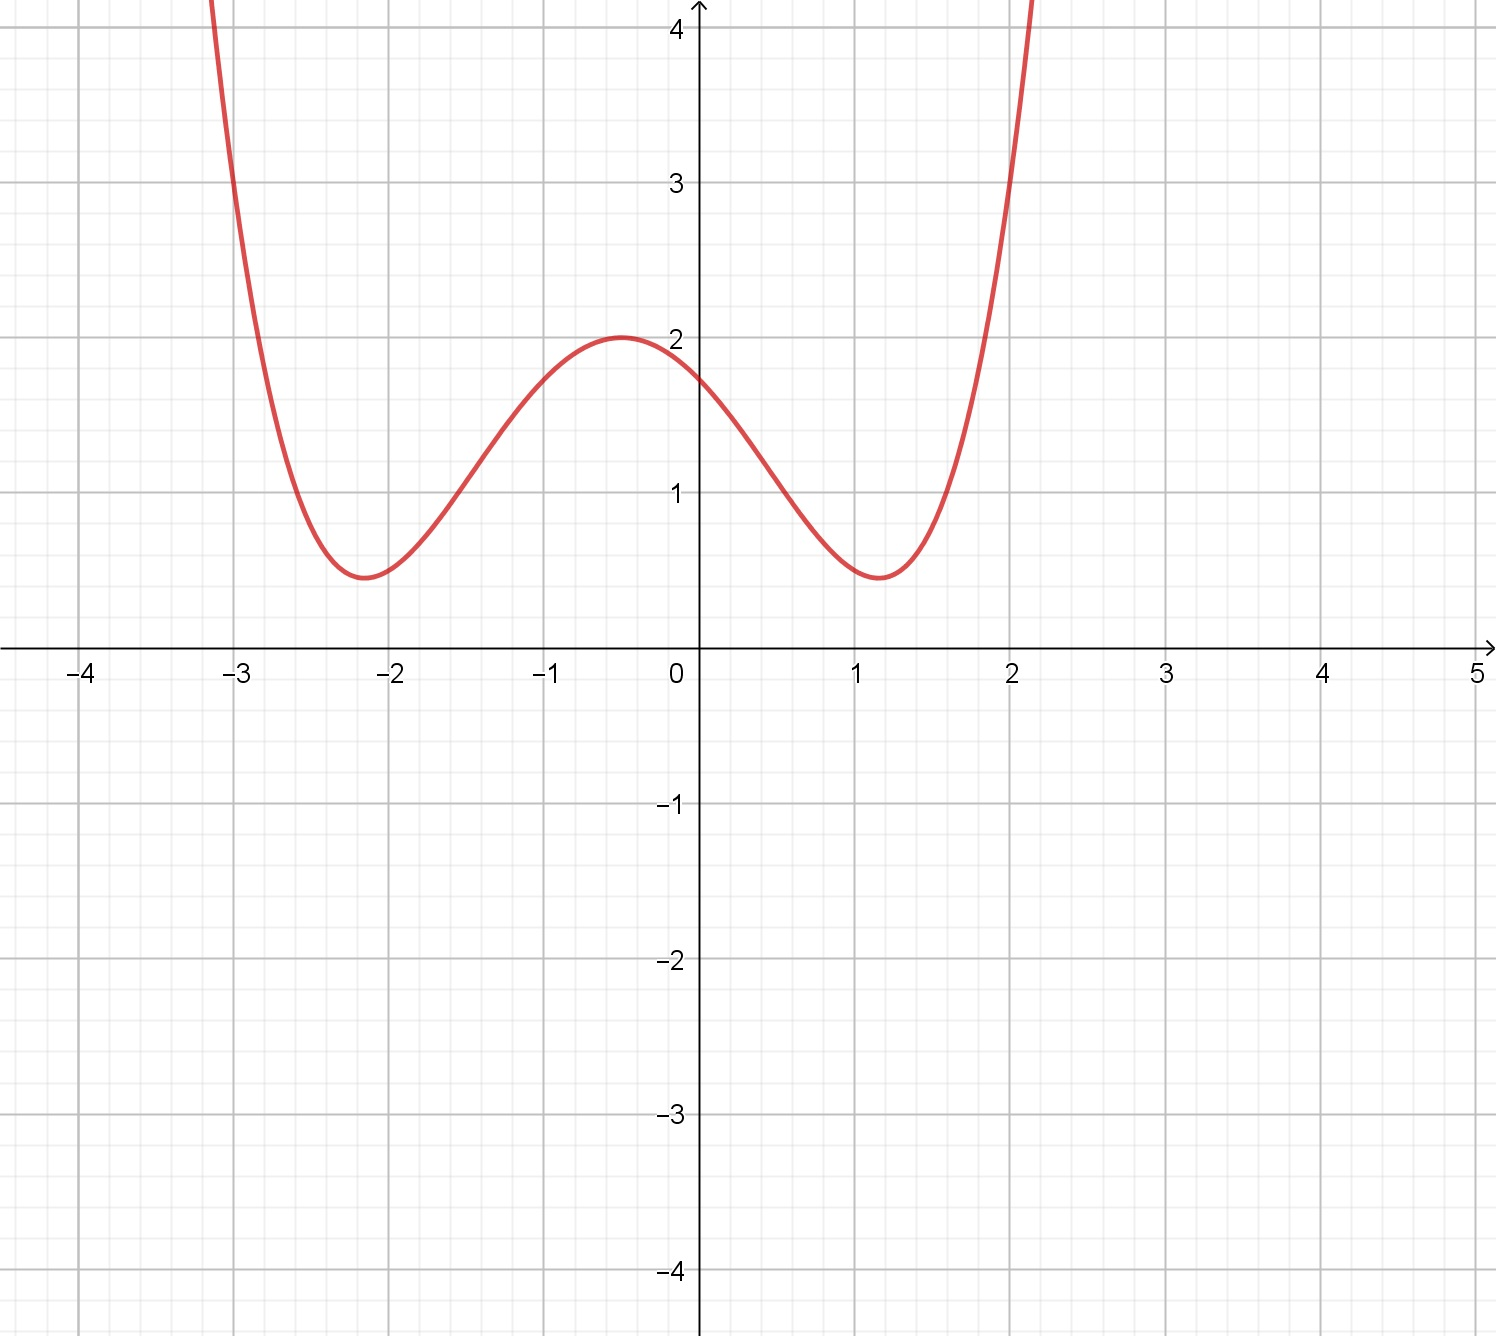
\includegraphics[scale=0.14]{../99_Bilder/3VKA/b.jpg} & & 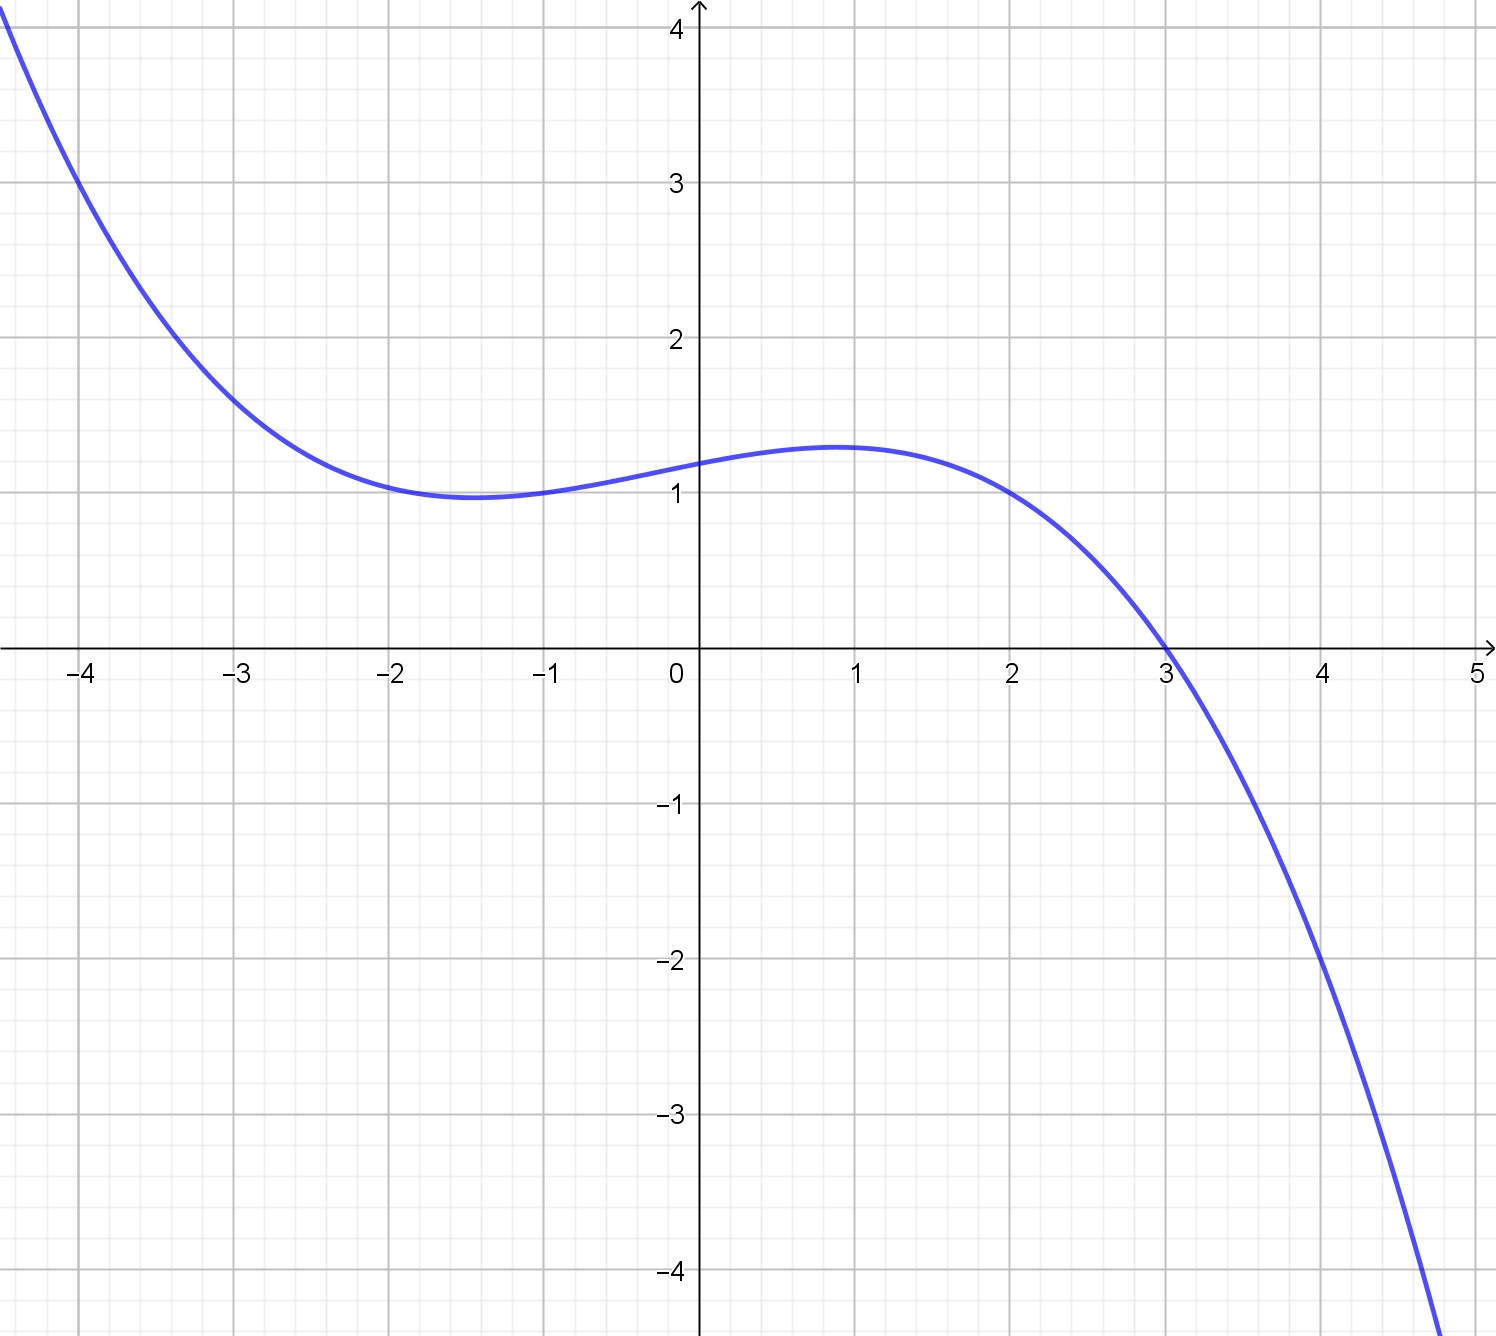
\includegraphics[scale=0.14]{../99_Bilder/3VKA/c.jpg}\\
		\hline
		\multicolumn{6}{|l|}{Graph der Steigungsfunktion}\\
		\hline
		(1) & & (2) & & (3) &\\
		& 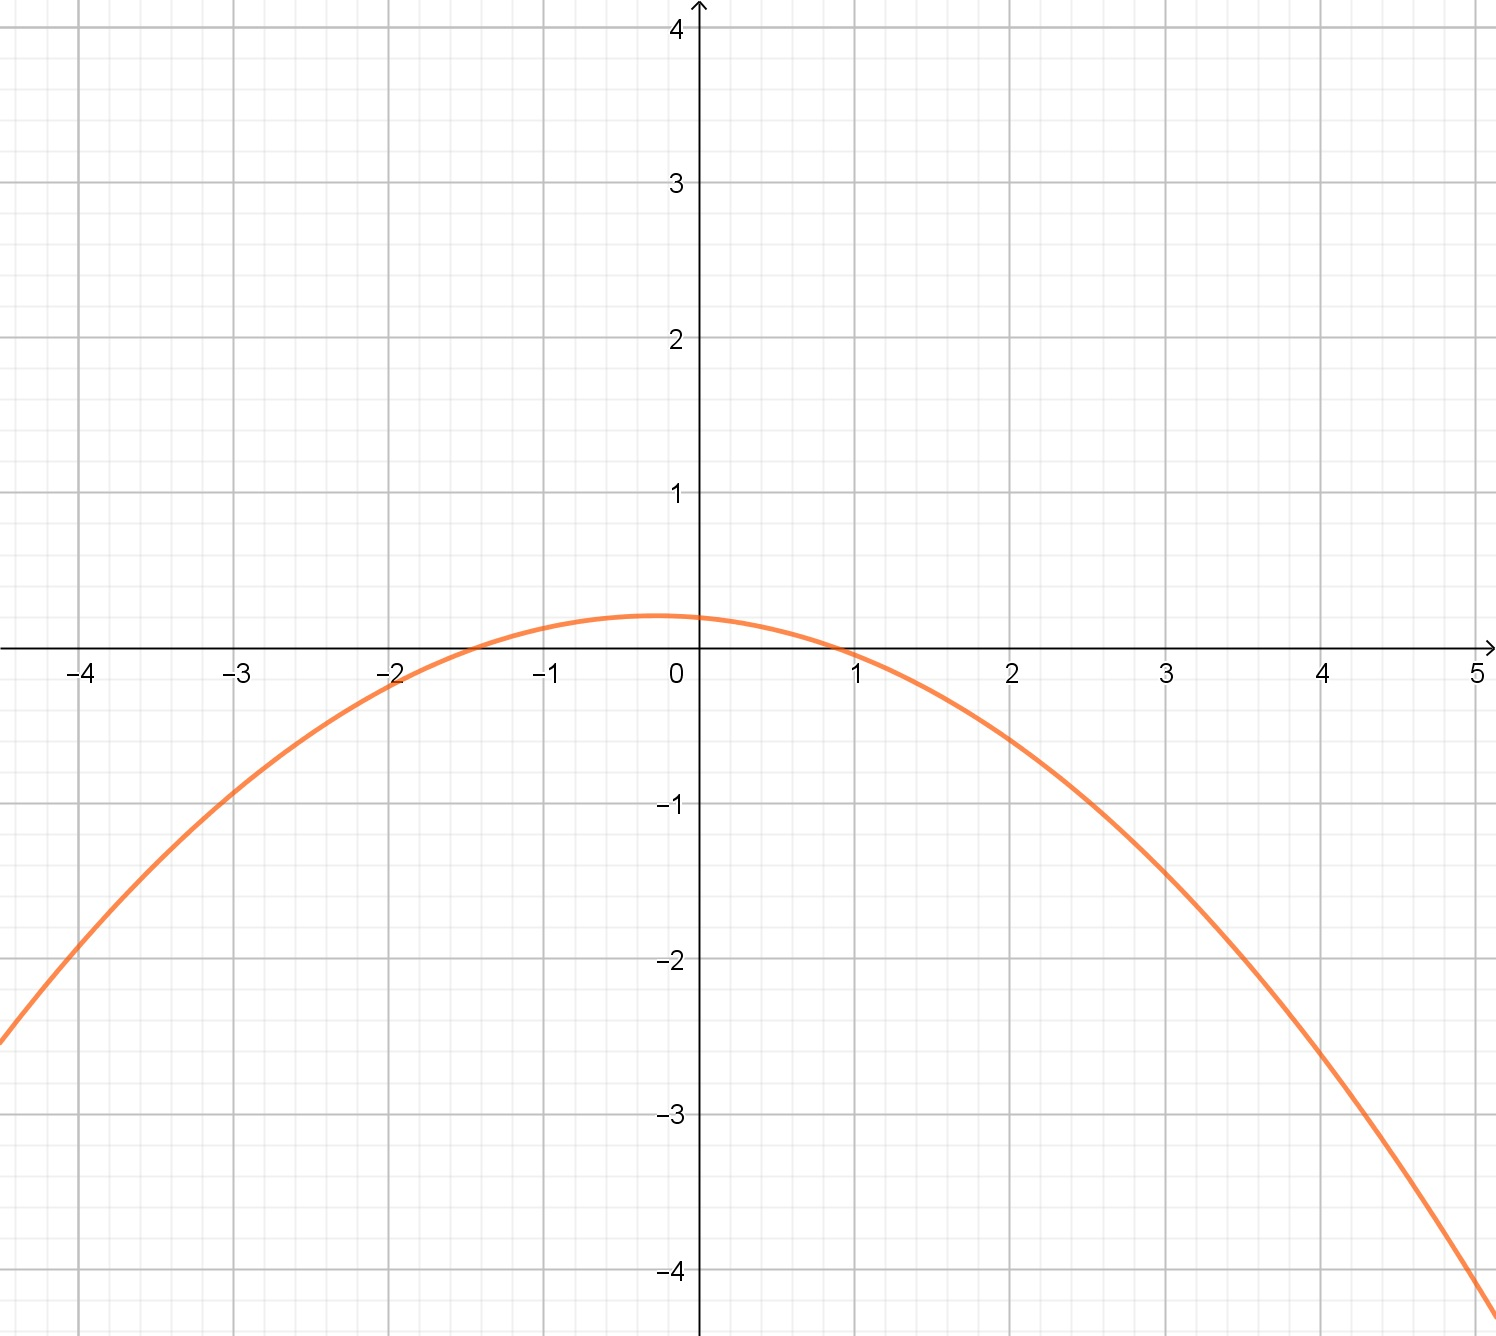
\includegraphics[scale=0.14]{../99_Bilder/3VKA/c-.jpg} & & 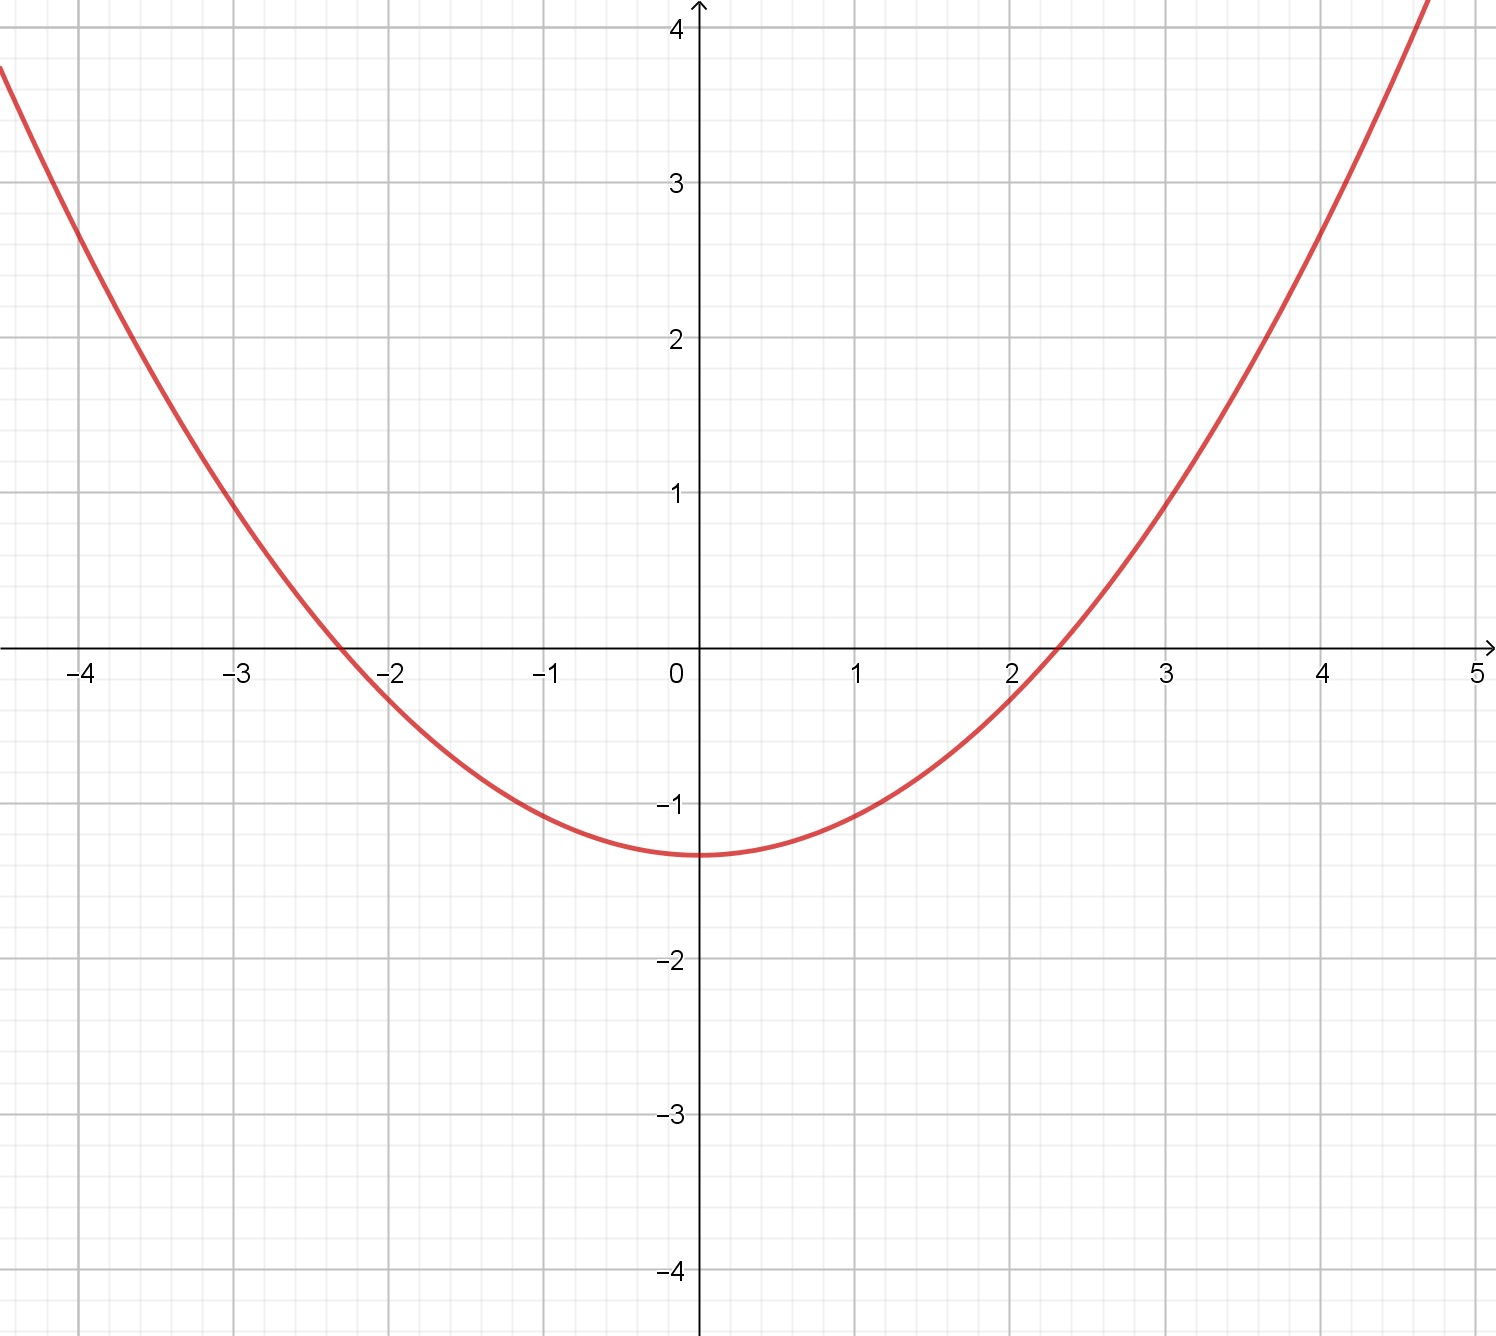
\includegraphics[scale=0.14]{../99_Bilder/3VKA/a-.jpg} & & 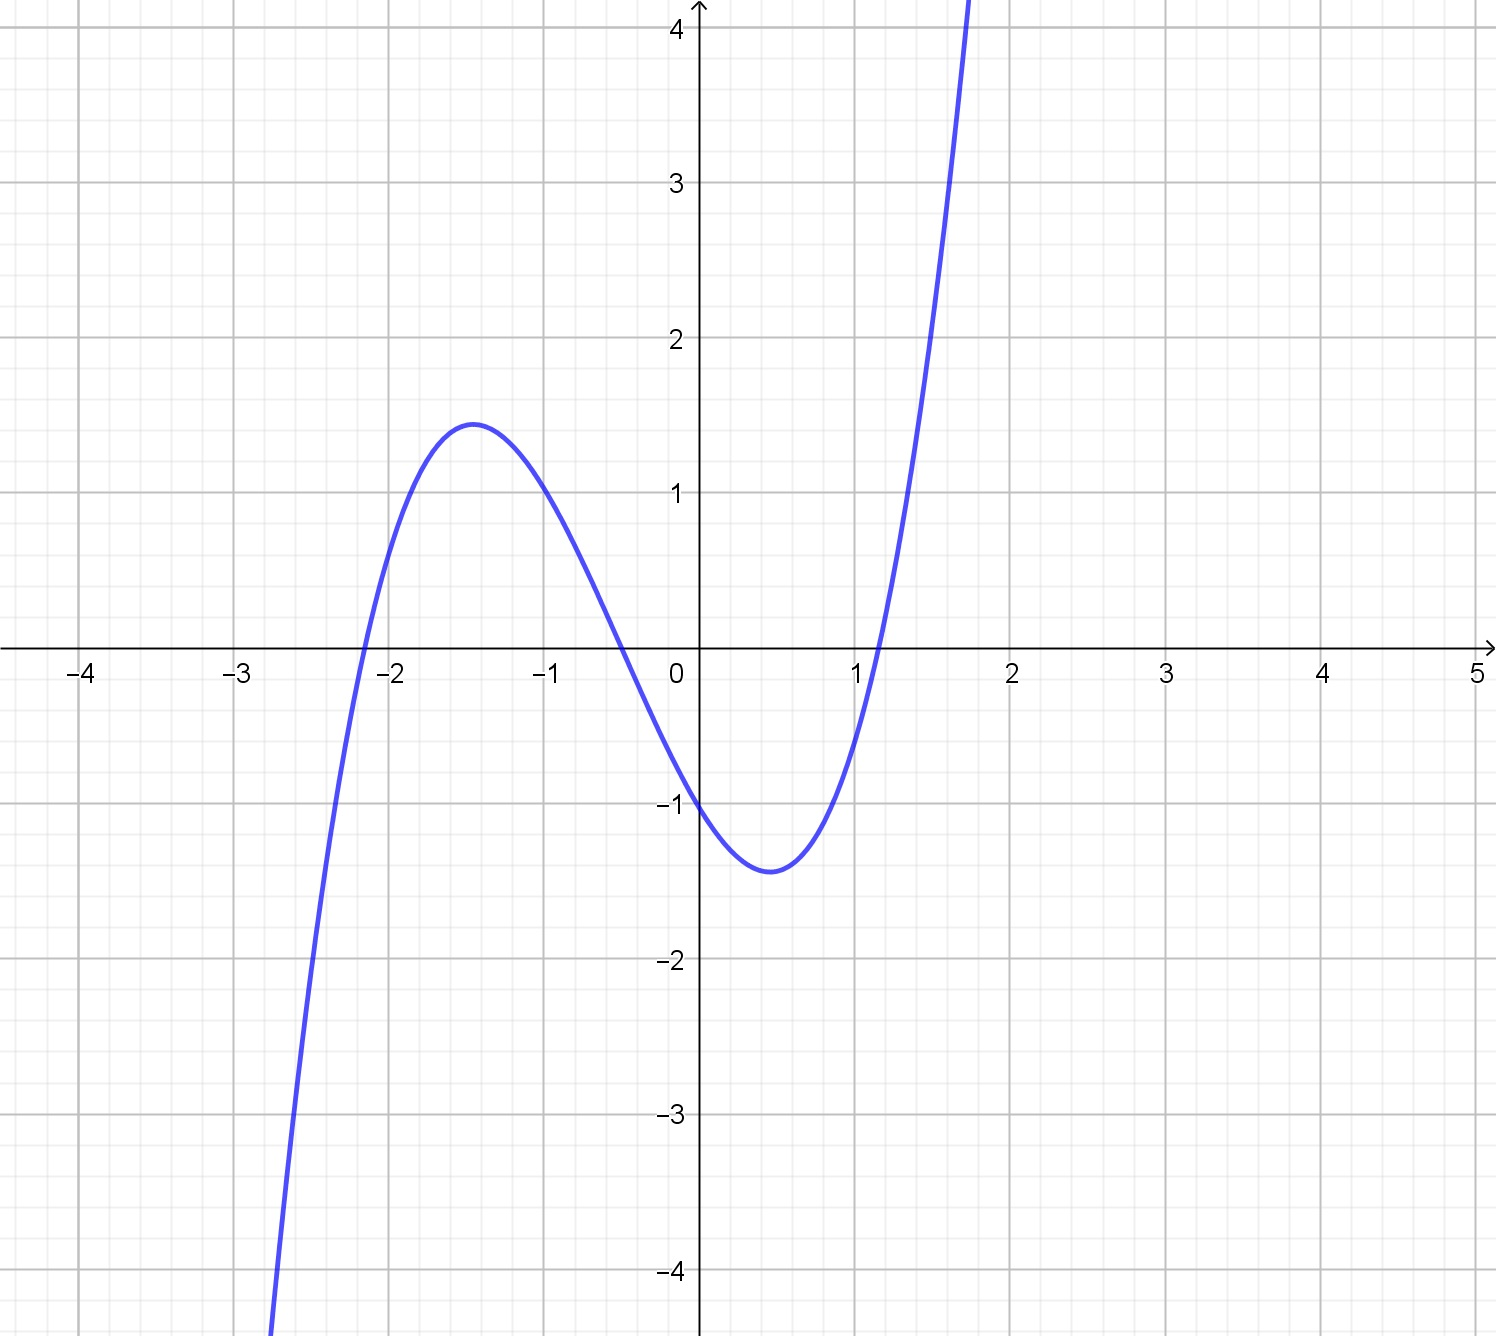
\includegraphics[scale=0.14]{../99_Bilder/3VKA/b-.jpg}\\
		\hline
	\end{tabularx}
	\par\noindent
	\begin{tabularx}{\textwidth}{Xl}\underline{\textbf{Aufgabe 5}}&\end{tabularx}\\
	\textbf{Bestimmen} Sie jeweils die \underline{Steigungsfunktion} der nachfolgenden Funktionen.
	\begin{itemize}
		\item[(I)] \(f(x) = 4x^4 + 5x^2 -2x\)
		\item[(II)] \(g(x) = -\frac{1}{3}x^3 - 2x + 3\)
		\item[(III)] \(h(x) = 0.5x^3 + \frac{1}{3}x^2 - 3x\)
	\end{itemize}
	\textbf{Berechnen} Sie zudem jeweils die \underline{Steigung} des Funktionsgraphen an den Stellen \(x_0 = 2\), \(x_0 = -1\) und \(x_0 = 0,5\).
\end{document}